\documentclass{TIJMUjiaoanSY}
\pagestyle{empty}


\begin{document}


%课程名称
\kecheng{Linux系统概论}
%实验名称
\shiyan{实验4\ Linux常用命令的操作}
%教师姓名
\jiaoshi{伊现富}
%职称
\zhicheng{讲师}
%教学日期(格式:XXXX年XX月XX日XX时-XX时)
\riqi{2018年5月28日13:30-15:30}
%授课对象(格式:XXX系XXXX年级XX班(硕/本/专科))
\duixiang{生物医学工程学院2016级生信班(本)}
%实验人数
\renshu{28}
%实验类型
\leixing{验证型}
%实验分组
\fenzu{一人一机}
%学时数
\xueshi{2}
%教材版本
\jiaocai{Linux系统概论上机指南(自编教材)}


%教案首页
\firstHeader
\maketitle
\thispagestyle{empty}

\mudi{
\begin{itemize}
  \item 了解监控系统性能的基本方法。
  \item 了解批量新建用户账户的步骤和方法。
  \item 理解/etc/passwd和/etc/group文件的含义。
  \item 掌握联机帮助页、命令选项的使用方法。
  \item 掌握目录和文件管理的常用命令。
  \item 掌握文件权限修改、归档和压缩的方法。
  \item 掌握输入输出重定向、管道、通配符和历史记录的使用方法。
  \item 掌握对文件内容进行排序的方法。
  \item 掌握利用shell命令管理用户和组的方法。
\end{itemize}
}

\fenpei{
\begin{itemize}
  \item (10')命令的帮助:总结查找命令帮助信息的四种方法。
  \item (5')命令的语法:介绍命令的基本语法。
  \item (5')命令的修改:回顾命令修改的知识点——通配符、输入输出重定向和管道。
  \item (80')实验操作:以CentOS发行版为例,练习基本命令的使用,掌握命令的基本语法。
\end{itemize}
}

\cailiao{
\begin{itemize}
  \item 主要仪器:一台安装有CentOS的计算机。
\end{itemize}
}

\zhongdian{
\begin{itemize}
  \item 重点难点:命令的基本语法,命令的修改。
  \item 解决策略:通过演示进行学习,通过练习熟练掌握。
\end{itemize}
}

\sikao{
\begin{itemize}
  \item 总结查看命令帮助的主要方法。
  \item 列举常见的通配符并解释其含义。
  \item 总结进行输入输出重定向的方法。
\end{itemize}
}

\cankao{
\begin{itemize}
  \item Linux基础及应用习题解析与实验指导(第二版),谢蓉\ 编著。中国铁道出版社,2014。
\end{itemize}
}

\firstTail


%教案续页
\newpage
\otherHeader

\noindent
\begin{enumerate}
  \item 命令的帮助(10分钟)
    \begin{enumerate}
\parpic[fr]{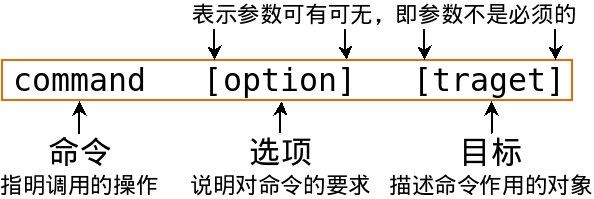
\includegraphics[width=8.5cm,height=2.3cm]{c4.command.png}}
      \item man:\textcolor{red}{联机帮助页},man cmd,man -k keyword
      \item info:信息帮助页,info cmd
      \item help:帮助信息,\verb|cmd --help|,cmd -h
      \item 其他:在线资源,等
    \end{enumerate}
  \item 命令的语法(5分钟)
\parpic[fr]{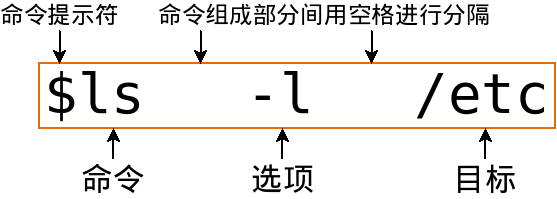
\includegraphics[width=8.5cm,height=2.5cm]{c4.command.ls.png}}
    \begin{enumerate}
      \item \textcolor{red}{基本语法}
        \begin{itemize}
	  \item Linux命令 = 命令 + [参数] 
	  \item 命令参数 = [选项] + [目标]
	  \item 分隔符:空格(Space)
	\end{itemize}
      \item 补充说明
	\begin{itemize}
\parpic[fr]{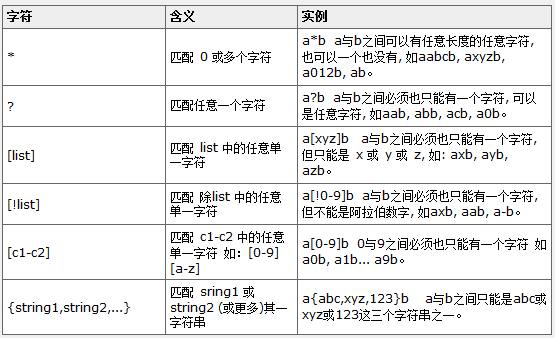
\includegraphics[width=8.5cm,height=6.2cm]{c4.metacharacter.png}}
	  \item 命令名与操作一致(ls: list)
	  \item 命令的默认行为(ls)
	  \item 参数影响输出格式和操作(-l /etc)
	  \item 目标提供处理目标(/etc)
	  \item 有些命令需要多个目标(cp OLD NEW)
	  \item 命令有独特的选项(ls -l)
	  \item 选项在一个或两个连字符后(-a = \verb|--all|)
	  \item 选项可以独立或是合并(-a -l = -al)
        \end{itemize}
    \end{enumerate}
  \item 命令的修改(5分钟)
    \begin{enumerate}
      \item 通配符:专用字符,能够用于同时匹配多个文件,从而增大一次性找到想要的文件名或目标的可能性。
	\begin{itemize}
	  \item \verb|*|:匹配任意长度的任何字符
	  \item \verb|?|:匹配一个字符
	  \item \verb|[]|:表示范围
	  \item \verb|-|:通常与\verb|[]|配合使用,起始字符-终止字符构成范围
	  \item \verb|!|:表示不在范围,通常也与\verb|[]|配合使用
	\end{itemize}
      \item 输入输出重定向
	\vspace*{-10pt}
	\begin{figure}[h]
	  \centering
	  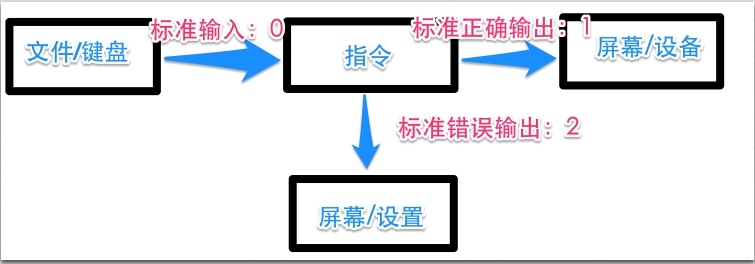
\includegraphics[width=7.5cm]{c4.io.01.jpg}
	  \quad
	  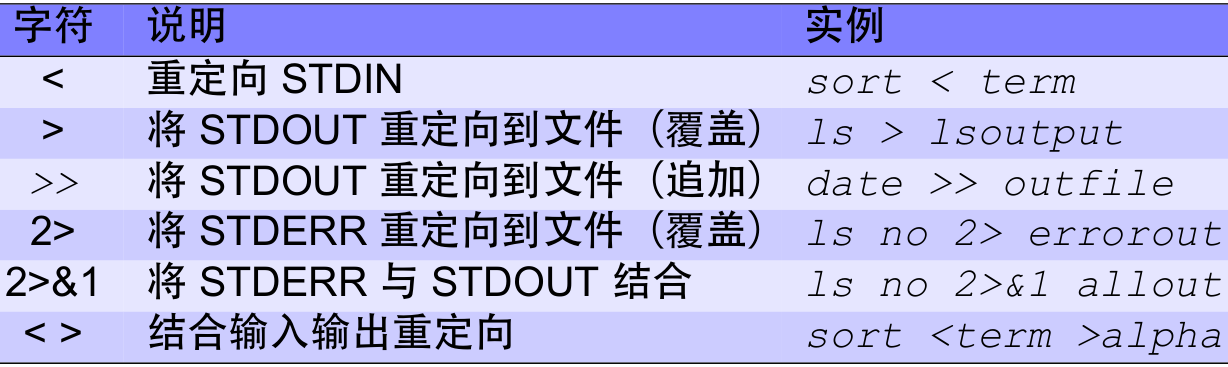
\includegraphics[width=9.3cm]{c4.io.png}
	\end{figure}
	\vspace*{-10pt}
      \item 管道
\parpic[fr]{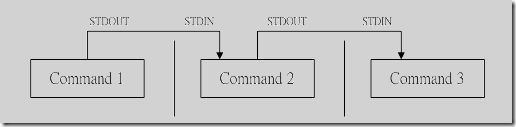
\includegraphics[width=8cm]{c4.pipe.png}}
	\verb=|=,一个操作符,把输入和输出重定向结合在一起,将一个命令的输出立即作为另一个命令的输入。
    \end{enumerate}
  \item 实验操作(80分钟)
    \begin{enumerate}
      \item 使用联机帮助页\textcolor{red}{(man -k permission; man chmod)}
      \item 命令选项\textcolor{red}{(ls -l -a /etc vs. ls -al /etc)}

\otherTail
\newpage
\otherHeader

      \item 文件管理
	\begin{itemize}
	  \item 目录操作:新建、切换、移动、删除、空间占用\textcolor{red}{(主要命令:mkdir,cd,mv,rm -rf,du)}
	  \item 文件操作:查找、修改权限、复制、创建链接\textcolor{red}{(主要命令:find,grep,chmod,cp,ln)}
	\end{itemize}
      \item 归档压缩
	\begin{itemize}
	  \item 压缩:tar\textcolor{red}{(主要选项:-czvf,-tf,--exclude,-N)},gzip
	  \item 解压缩:tar\textcolor{red}{(主要选项:-xzvf)},gunzip
	\end{itemize}
      \item 系统监控:top\textcolor{red}{(主要命令:M,P,h,q)}
      \item 通配符\textcolor{red}{(*,?,[],-,!)}
      \item 历史命令\textcolor{red}{(主要命令:history,!!)}
      \item 文本排序:sort\textcolor{red}{(主要选项:-d,-u)}
      \item 用户和组管理
	\begin{itemize}
	  \item 用户管理\textcolor{red}{(主要命令:useradd,passwd,id,su,userdel)}
	  \item 组管理\textcolor{red}{(主要命令:groupadd,groupmod,groupdel)}
	\end{itemize}
      \item 批量新建用户账户
	\begin{itemize}
	  \item 新建共同组\textcolor{red}{(主要命令:groupadd)}
	  \item 创建用户信息文件\textcolor{red}{(/etc/passwd格式)}
	  \item 创建用户密码文件
	  \item 批量新建用户\textcolor{red}{(主要命令:newusers,pwunconv,chpasswd,pwconv)}
	\end{itemize}
    \end{enumerate}
\end{enumerate}


\otherTail


\end{document}

